\paragraph{Activation Functions} \label{sec:activation}

Activation functions are essential to neural networks, as they introduce non-linearity into the model. Nonlinearity is important because it allows the model to learn complex relationships between inputs and outputs. This section will discuss some of the most commonly used activation functions, including sigmoid, \ac{tanh}, and \ac{ReLU}.

\begin{figure}[ht]
    \centering
    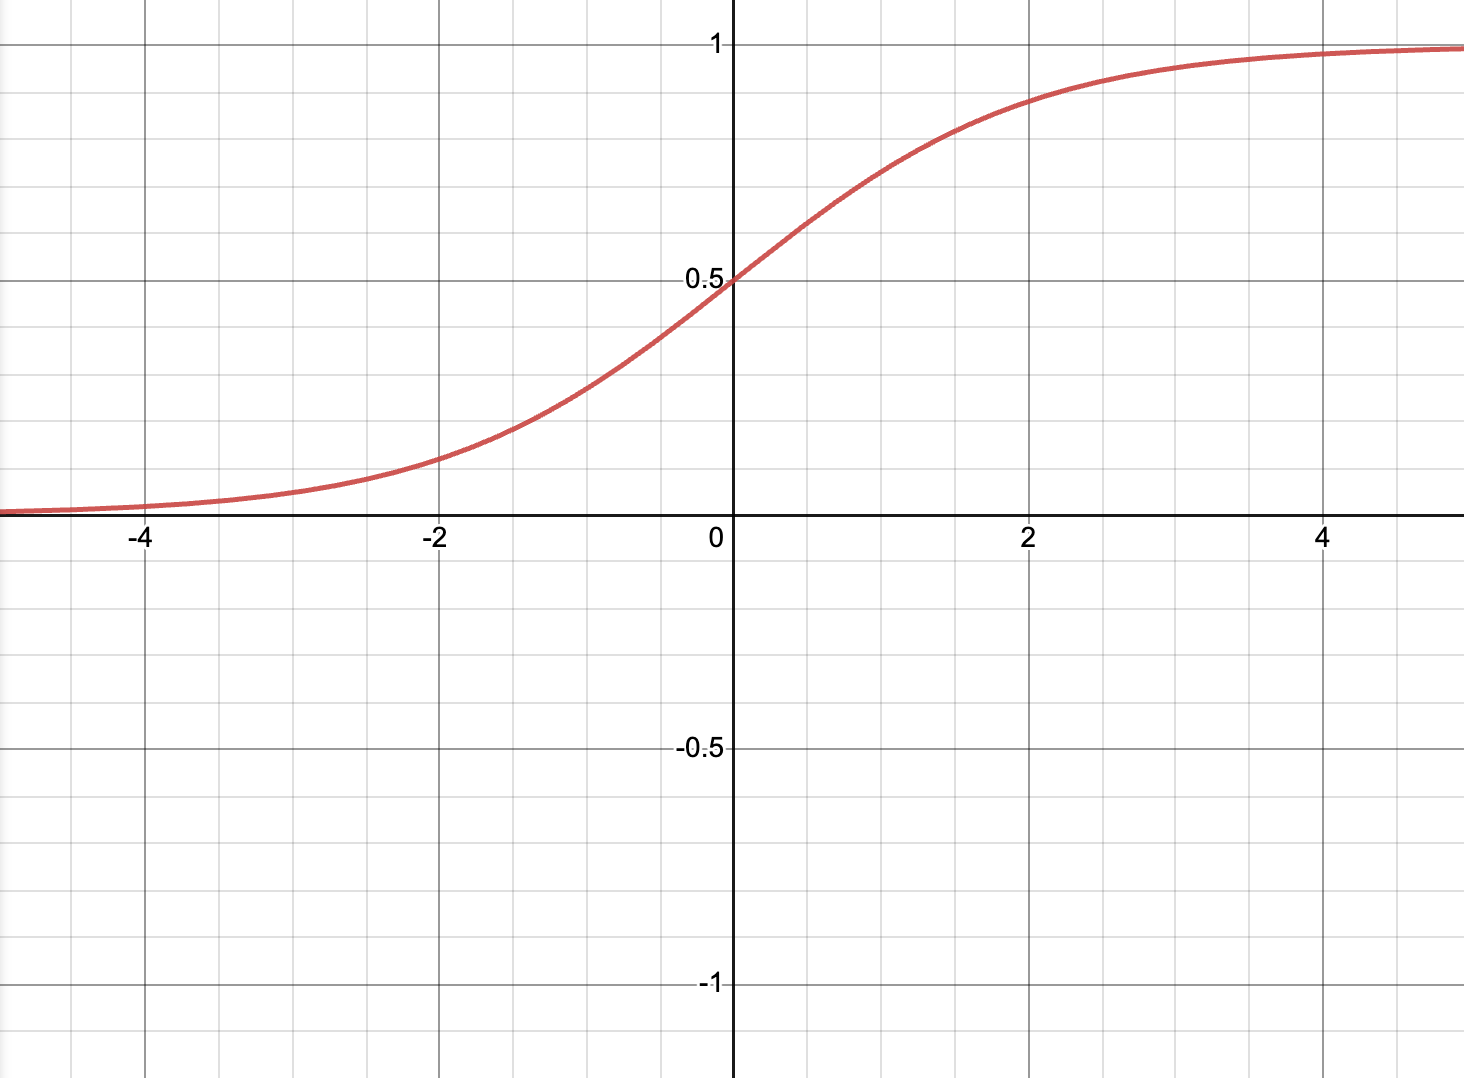
\includegraphics[width=\textwidth/2]{figures/2-sota/activation/sigmoid.png}
    \caption[Sigmoid Activation Function]{One can see that the values that are output are exclusively between 0 and 1 with its value being 0.5 for $x = 0$.}
    \label{fig:sigmoid}
\end{figure}

\label{sec:sigmoid}

The \textbf{sigmoid} activation function is prevalent in neural networks. It is defined as:

\begin{equation}
	\sigma(x) = \frac{1}{1 + e^{-x}}
\end{equation}

where $x$ is the input to the function. The output of the sigmoid function is always between 0 and 1, which makes it useful for binary classification tasks. The sigmoid function is also differentiable, which is essential for backpropagation during training. Figure \ref{fig:sigmoid} visually represents this function.

However, the sigmoid function has a few drawbacks. One issue is that the function's gradient approaches zero as the input becomes very large or very small. This can cause the weights to update very slowly during training, a problem known as the \textit{vanishing gradient} problem. Additionally, the output of the sigmoid function is not zero-centered, which can make optimization more difficult. On the other hand, if the gradients become extremely large, it can cause the weights to update too much in each iteration, leading to the \textit{gradient explosion problem}. This can lead to the model diverging and failing to converge to a good solution. 

\label{sec:tanh}

The \textbf{\acf{tanh}} activation function is similar to the sigmoid function, but its output is between -1 and 1:

\begin{equation}
	\tanh(x) = \frac{e^x - e^{-x}}{e^x + e^{-x}}
\end{equation}

Tanh is differentiable and valuable for binary classification tasks like the sigmoid function. However, it has the same vanishing gradient problem as the sigmoid function. A visual representation can be seen in Figure~\ref{fig:tanh}.

\begin{figure}[ht]
    \centering
    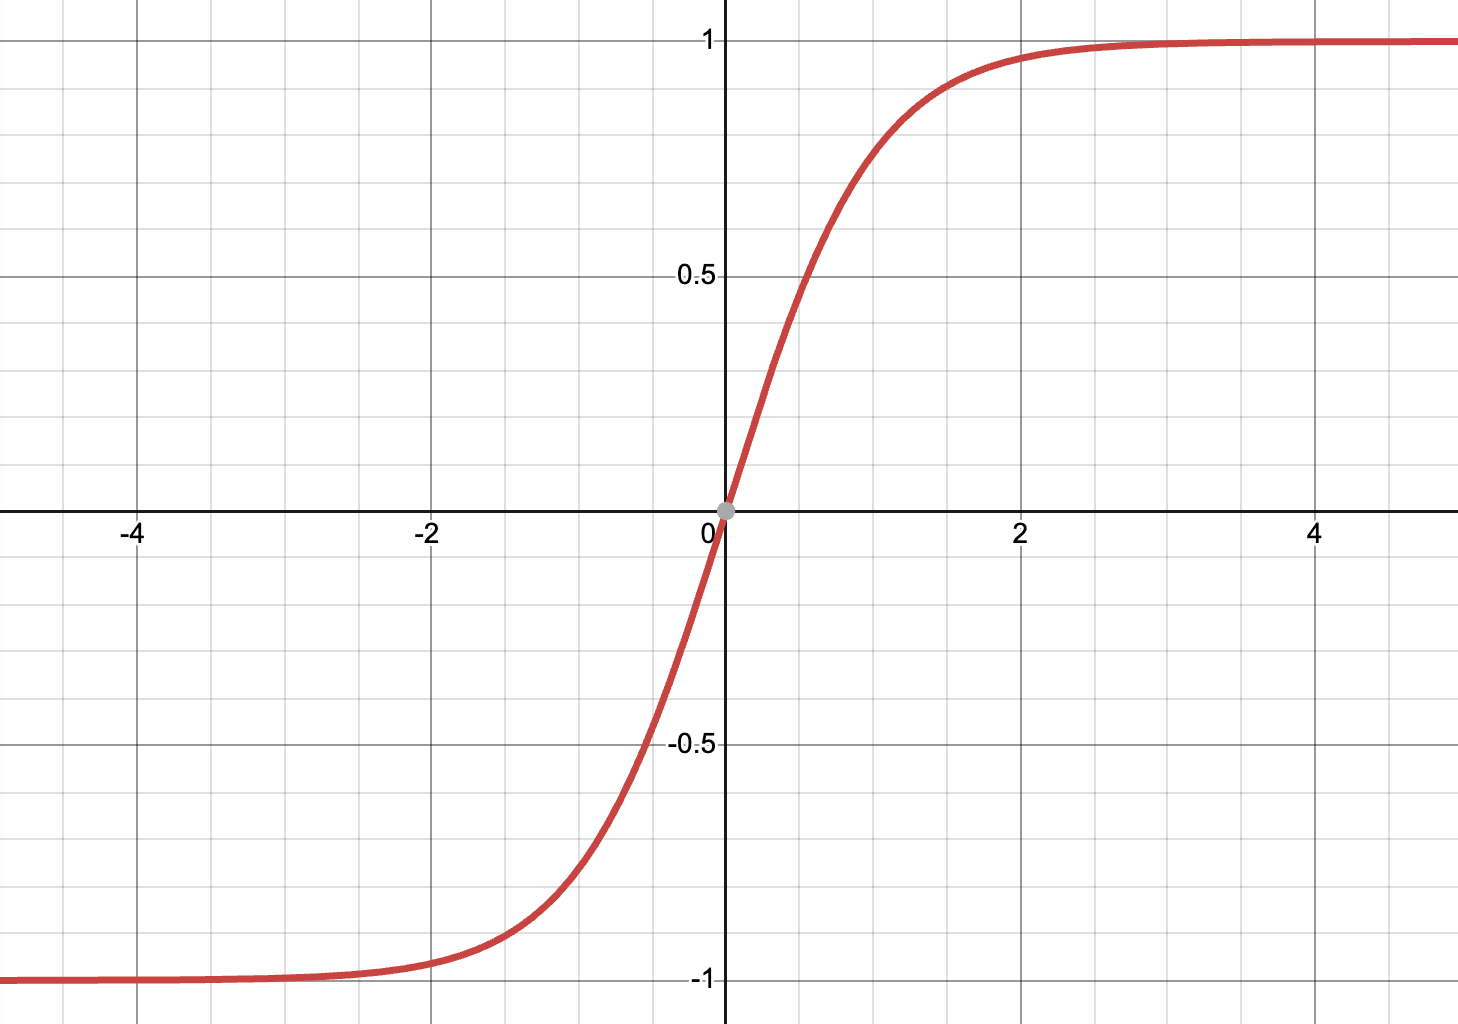
\includegraphics[width=\textwidth/2]{figures/2-sota/activation/tanh.png}
    \caption[Tanh Activation Function]{A very similar function except that its limits are present on -1 and 1}
    \label{fig:tanh}
\end{figure}

\label{sec:relu}

The \textbf{\acf{ReLU}} activation function is a popular choice in \ac{DL}. It is defined as:

\begin{equation}
	\text{ReLU}(x) = \max(0, x)
\end{equation}

The \ac{ReLU} function is also zero-centered, which can make optimization easier. However, this function is not differentiable at $x=0$, which can cause problems during training. Variants of the \ac{ReLU} function have been proposed to address this issue. A visual representation can be seen in Figure \ref{fig:relu}.

\begin{figure}[ht]
    \centering
    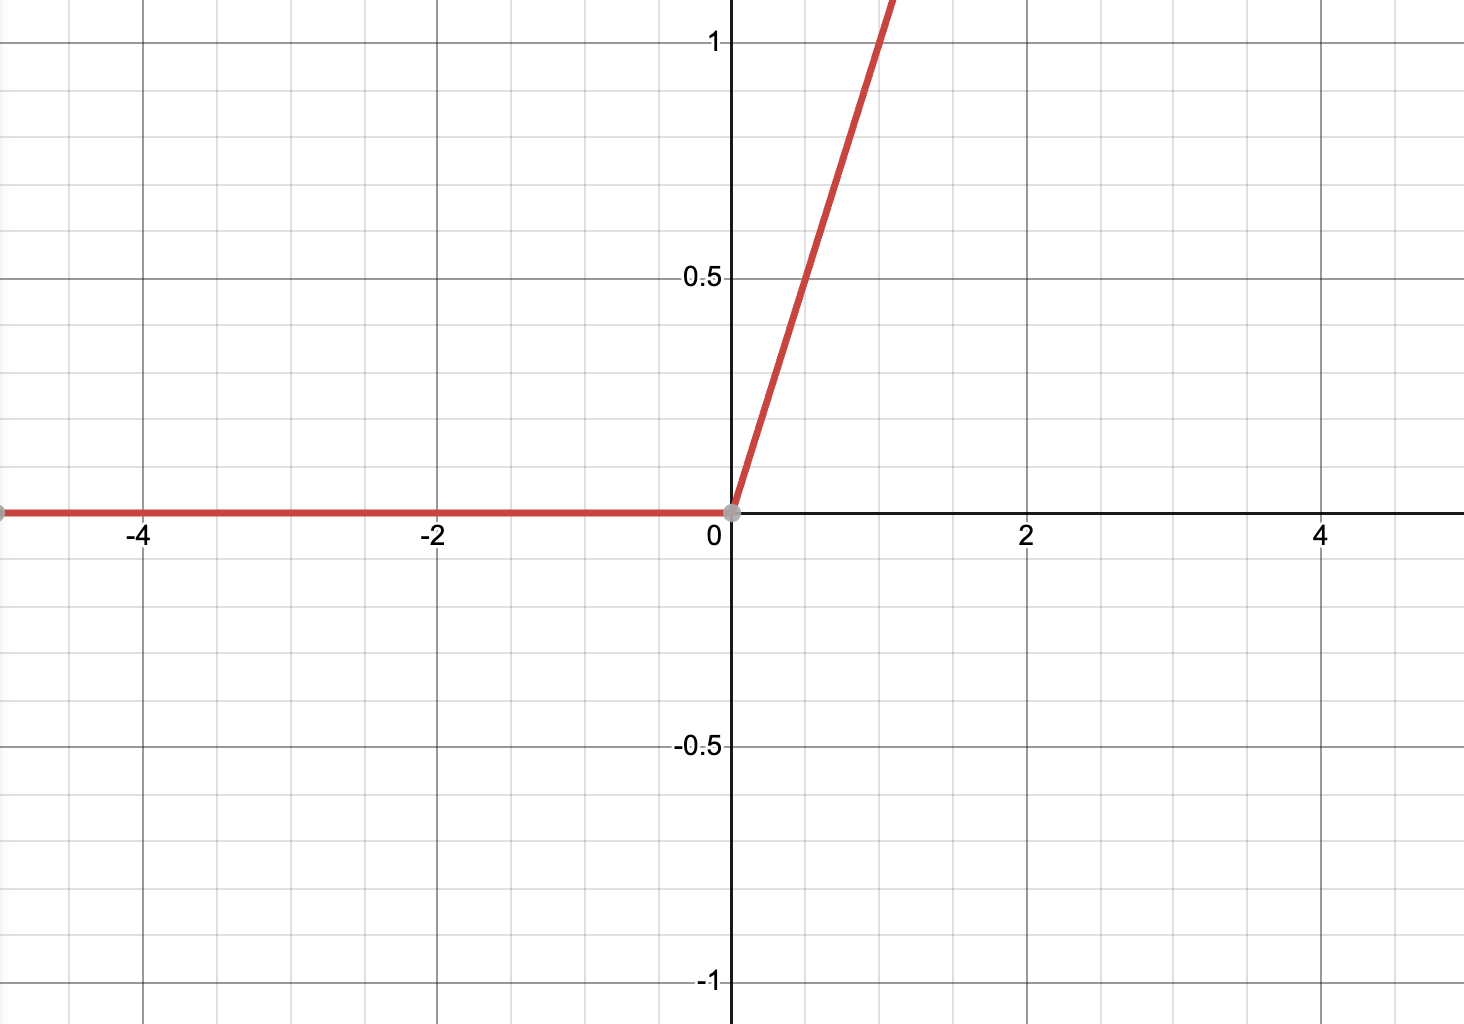
\includegraphics[width=\textwidth/2]{figures/2-sota/activation/relu.png}
    \caption[Relu Activation Function]{Linear for positive values, 0 for negative values.}
    \label{fig:relu}
\end{figure}

The \ac{ReLU} activation has a potential problem known as the \textit{dying ReLU} problem. When a neuron's weights become such that its input is always negative, its gradient will always be zero. In this situation, the neuron will become inactive, or \textit{dead}, and will no longer update during training. This problem can lead to underfitting, as some neurons stop learning and contributing to the model. Variants of \ac{ReLU}, such as \textbf{Leaky \ac{ReLU}}, have been proposed to mitigate the dying \ac{ReLU} problem by assigning a slight non-zero gradient for negative input values.

The Leaky ReLU function is defined as:

\begin{equation}
\text{Leaky ReLU}(x) = \text{max}(a x , x)
\end{equation}

where $a$ is a small positive number such as $0.01$. This non-zero gradient for negative inputs can help prevent neurons from becoming inactive during training. This function can visually be seen in Figure~\ref{fig:leaky-relu}.

\begin{figure}[ht]
    \centering
    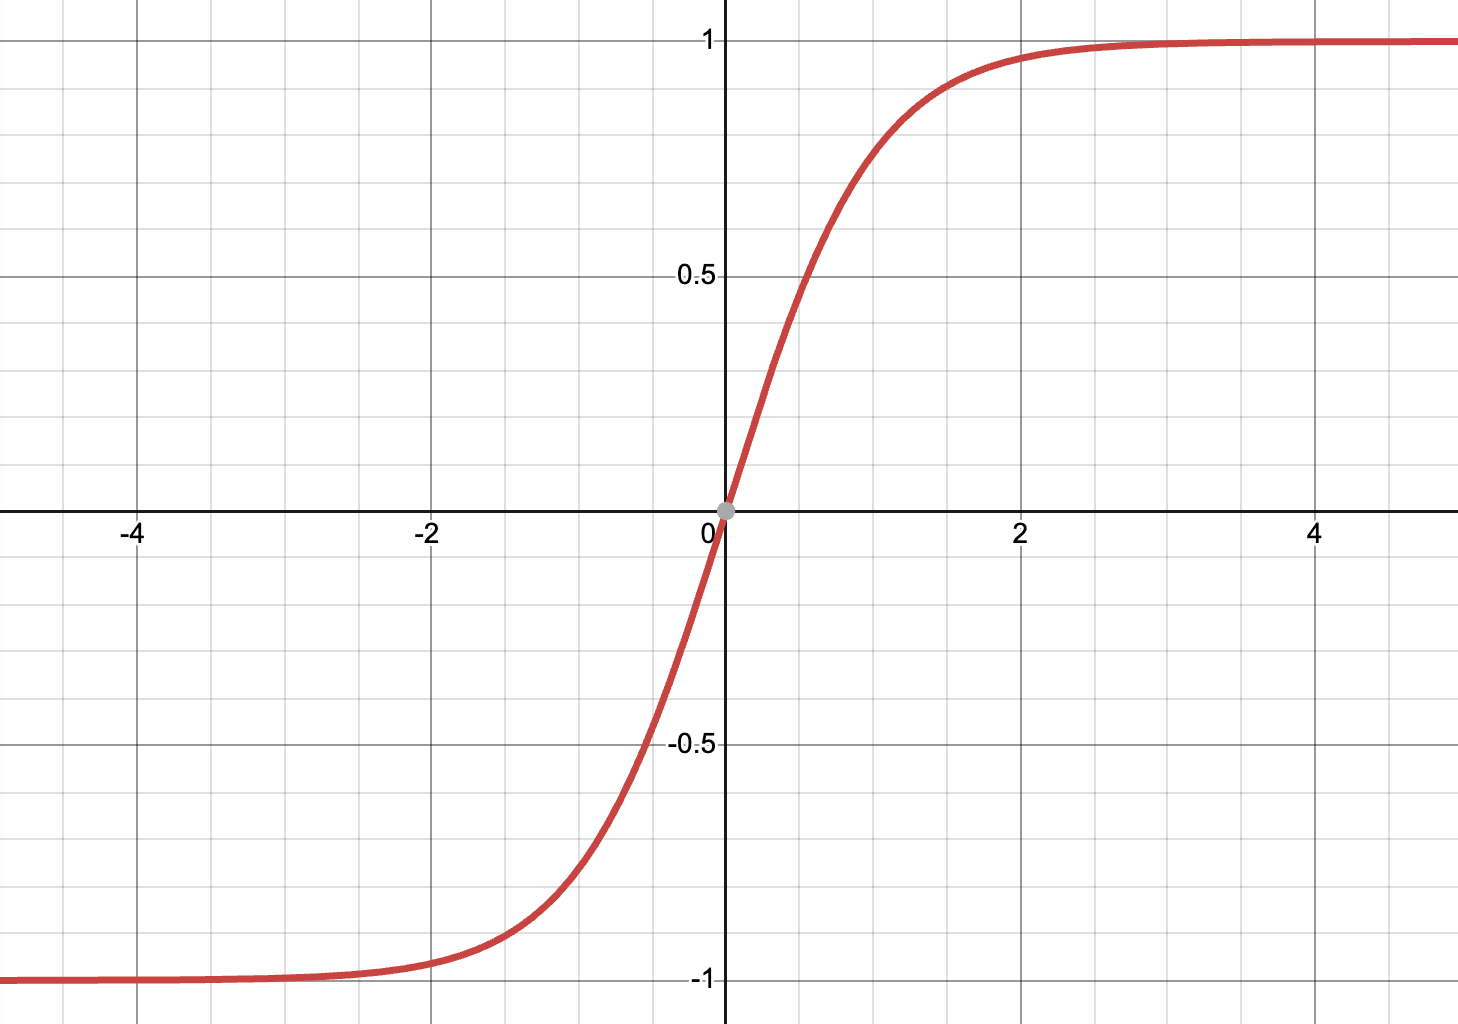
\includegraphics[width=\textwidth/2]{figures/2-sota/activation/tanh.png}
    \caption[Leaky Relu Activation Function]{Very similar to Relu but with non-zero gradient for negative inputs.}
    \label{fig:leaky-relu}
\end{figure}